\subsection{Preprocesamiento De Los Datos} 
Con el objetivo de darle mayor estabilidad matematica a los datos y quitar algo del ruido que puedan tener, realizamos un preprocesamiento de los mismos. El mismo consistió en quitar los utliers dentro del set de datos y luego normalizarlos con media 0 y varianza 1.

\subsection{Implementacion Del algoritmo} 

El algoritmo que implementamos consistió en una red neuronal profunda con retropropagación del error. Este, descripto de manera informal consiste en introducir una instancia del problema, calcular la salida, compararla con la salida esperada y retropropagar el error, con el objetivo modificar las matrices de pesos y minimizar la diferencia. El sistema implementado se dice ser $online$ ya que los pesos de las matrices son ajutados luego de retropropagar el error de cada instancia en vez de hacerlo al final de la epoca.

A fin de tener una medida de como va \"aprendiendo\" la red neuronal, luego de presentarle a la red todas las instancias una vez, calculamos la norma de la diferencia entre las respuestas obtenidas y las esperadas. Consideraremos esta nuestra "norma del error" y la tomaremos como una metrica adecuada para saber cuan buenos resultados devuelve nuestra red.

%habria que poner pseudocodigo o algo mas lindo acá
%Aprovechando este calculo de la norma, decidimos agregar a la implementación, un learning rate adaptativo. El mismo consiste en, en caso de que la norma haya decrecido, aumentar el learnin rate. En caso contrario, es decir, la norma del error aumentó, quiere decir que la red empeoro la solucion y decrecemos el learnig rate.

Como optimización adicional se agrego un termino de momentum. La idea tras esto consiste en darle a cada peso de la matriz una "inercia" que le permita continuar avanzando en la direccion en la que avanzó en la iteración anterior. El objetivo consiste en disminuir las oscilaciones con cada pequeño cambio en la matriz.

\subsection{Convergencia del algoritmo en Diagnostico de Cancer} 

Para este problema utilizaremos una neurona en la ulima capa con función de activación logistica. Para ser consistentes con esto, las salidas esperadas adoptarán los valores $1$ si resulto ser cancer maligno, y $0$ si resulto ser benigno. La experimentación consistirá en buscar los parametros optimos que nos den la mayor tasa de aciertos para nuestro data set.

Como primera instancia comprobaremos que la red converge efectivamente a la solución esperada. Para eso tomamos un lerning rate de $0.01$ y con $1300$ epocas graficamos la norma del error cada $1000$ iteraciones:

\begin{figure}[h!]
  \centering
    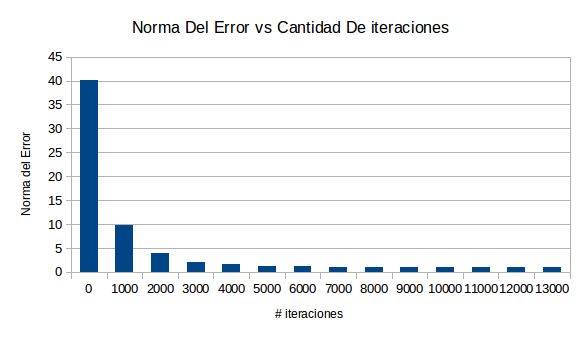
\includegraphics[scale=0.4]{ej1_convergencia/1.png}
\end{figure}

El grafico muestra que, efectivamente, nuestro algoritmo minimiza la diferencia entre las soluciones obtenidas y las deseadas, minimizando así tambien la norma del error.

\subsection{Variación de los resultados variando el learning rate} 

Para evitar el sobreajuste las experimentaciones todas las experimentaciones desde este punto se realizarán con la siguente metodología. Se dividirá el set de datos de entrenamiento provisto por la catedra en dos sets de datos distintos. Uno se utilizará para entrenar la red, mientras que el otro se medirán que tan buenos fueron los resultados obtenidos. Con esto se espera reducir el overfittning que la red pueda generar y comprobar de manera mas acertada que tan buenos resultados dará la red sobre datos reales del problema.

\reescribir 

En esta sección querremos experimentar es como se comporta el algoritmo al variar el learning rate. Para ello, dejamos constantes las cantidad de epocas de entrenamiento en $10000$ y variamos el learning desde $0.01$ hasta $0.2$ aumentando de a $0.01$
%Capaz va mas arriba?

\begin{figure}[h!]
  \centering
    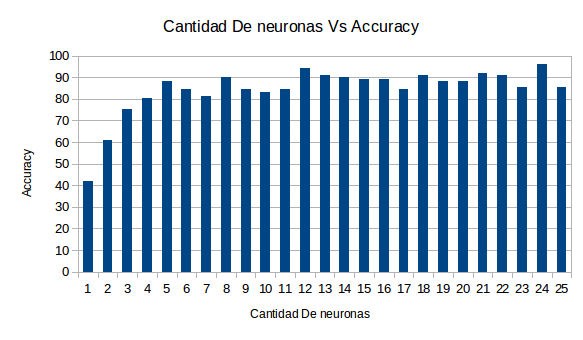
\includegraphics[scale=0.4]{ej1/cantNeuronasVsAccuracy.png}
\end{figure}

Puede verse en el grafico que para $13$ neuronas el modelo consigue un acuracy aproximado del $90\%$, pareciendo este ser el maximo alcanzable para los parametros fijados. Luego seteamos este valor y pasamos a variar el learning rate, dejando todos los otros parametros constantes:

\begin{figure}[h!]
  \centering
    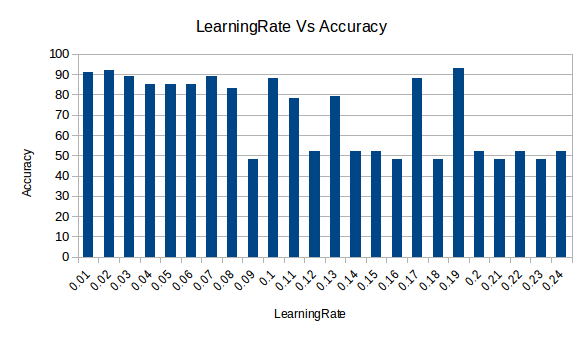
\includegraphics[scale=0.4]{ej1/learningRate.png}
\end{figure}

En el grafico puede obsercarse que aumentando demasiado el learning rate los resultados parecen volverse peores, asi que lo seteamos en un valor igual a $0.02$.

Por ultimo variamos la cantidad de epocas para ver como se ve afectado el aprendisaje de la red neuronal, dejando los parametros seteados como ya hemos mencionado previamente:

\begin{figure}[h!]
  \centering
    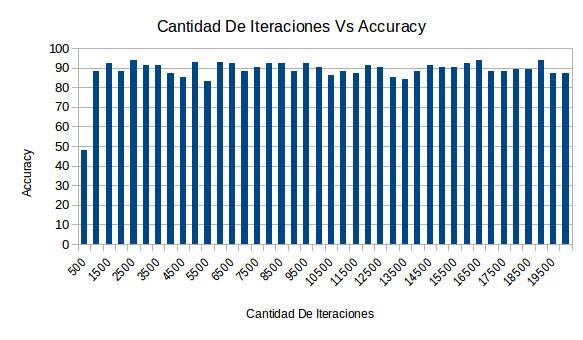
\includegraphics[scale=0.4]{ej1/iteraciones Vs accuracy.png}
\end{figure}

Puede verse que ya para $1500$ epocas el algoritmo ya alcanza un maximo de $90\%$ acuracy.

\subsection{Performance Regreción Lineal Calor} 

%falta implementar
Por cuestiones de tiempo este ejercicio no fue probado de manera adecuada